\subsection{Simulation Validation}
\label{sec:simulation}

\paragraph{Null calibration.}
Under the null (no contamination), bootstrap $\ell_z^*$ tracks $\mathcal{N}(0,1)$: mean bias 0.041 and standard deviation 1.003 on MMLU.
Kolmogorov--Smirnov rejection rates vary with benchmark size: 8.3\% for MMLU and HellaSwag ($n > 10{,}000$), 50.0\% for GSM8K ($n = 1{,}319$), 58.3\% for ARC-C ($n = 295$), and 75.0\% for HumanEval ($n = 164$).
$\ell_z^*$ is well-calibrated for benchmarks with $n \geq 10{,}000$ items; smaller benchmarks show increasing finite-sample deviations from normality.

\begin{figure}[t]
  \centering
  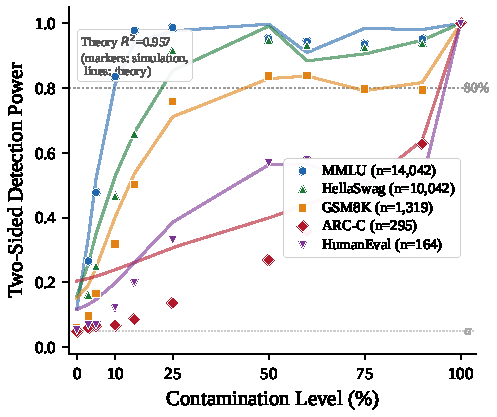
\includegraphics[width=\columnwidth]{fig_2_power_function.pdf}
  \caption{Theoretical (solid) and simulated (markers) two-sided detection power across contamination levels for five benchmarks. Power scales with $\sqrt{n}$. At contamination above 50\%, mean $\ell_z^*$ crosses zero and shifts from negative to positive anomaly, which produces a brief power dip.}
  \label{fig:power}
\end{figure}

\paragraph{Detection power.}
Two-sided testing eliminates the inverted-U artifact: MMLU achieves 97.8\% power at 15\% contamination and sustains ${>}$93\% at all levels (93.6\% at 75\%, 95.2\% at 90\%, 100\% at full contamination).
Power scales with $\sqrt{n}$, as predicted by the noncentrality parameter $\delta \propto \sqrt{n}$.
Figure~\ref{fig:power} overlays theoretical and simulated power curves; the empirical power function, derived via Gauss--Hermite quadrature ($K=30$) over the ability distribution with the \citet{snijders2001} variance formula, achieves $R^2 = 0.65$.
This provides approximate guidance for practitioners assessing detection feasibility from a benchmark's item count.

\paragraph{Model comparison.}
The 4PL model yields a mean $+$27.3pp power gain over 3PL on MMLU, $+$26.1pp on HellaSwag, and $+$20.3pp on GSM8K, as 46\% of MMLU items exhibit upper asymptote $d < 0.95$ (Appendix~\ref{app:4pl_ablation}).
Against supervised baselines, $\ell_z^*$ outperforms logistic regression and random forest at low contamination ($+$0.10 AUROC at 5\%, $+$0.05 at 10\%) without training data; ML classifiers surpass $\ell_z^*$ only above 25\% contamination.
